\documentclass[11pt]{article}
\usepackage{fullpage}
\usepackage{amsmath}
\usepackage{amssymb}
\usepackage{graphicx}

\title{Template}
\author{Name}
\begin{document}

\subsection*{Problem 4}
Part a.)

    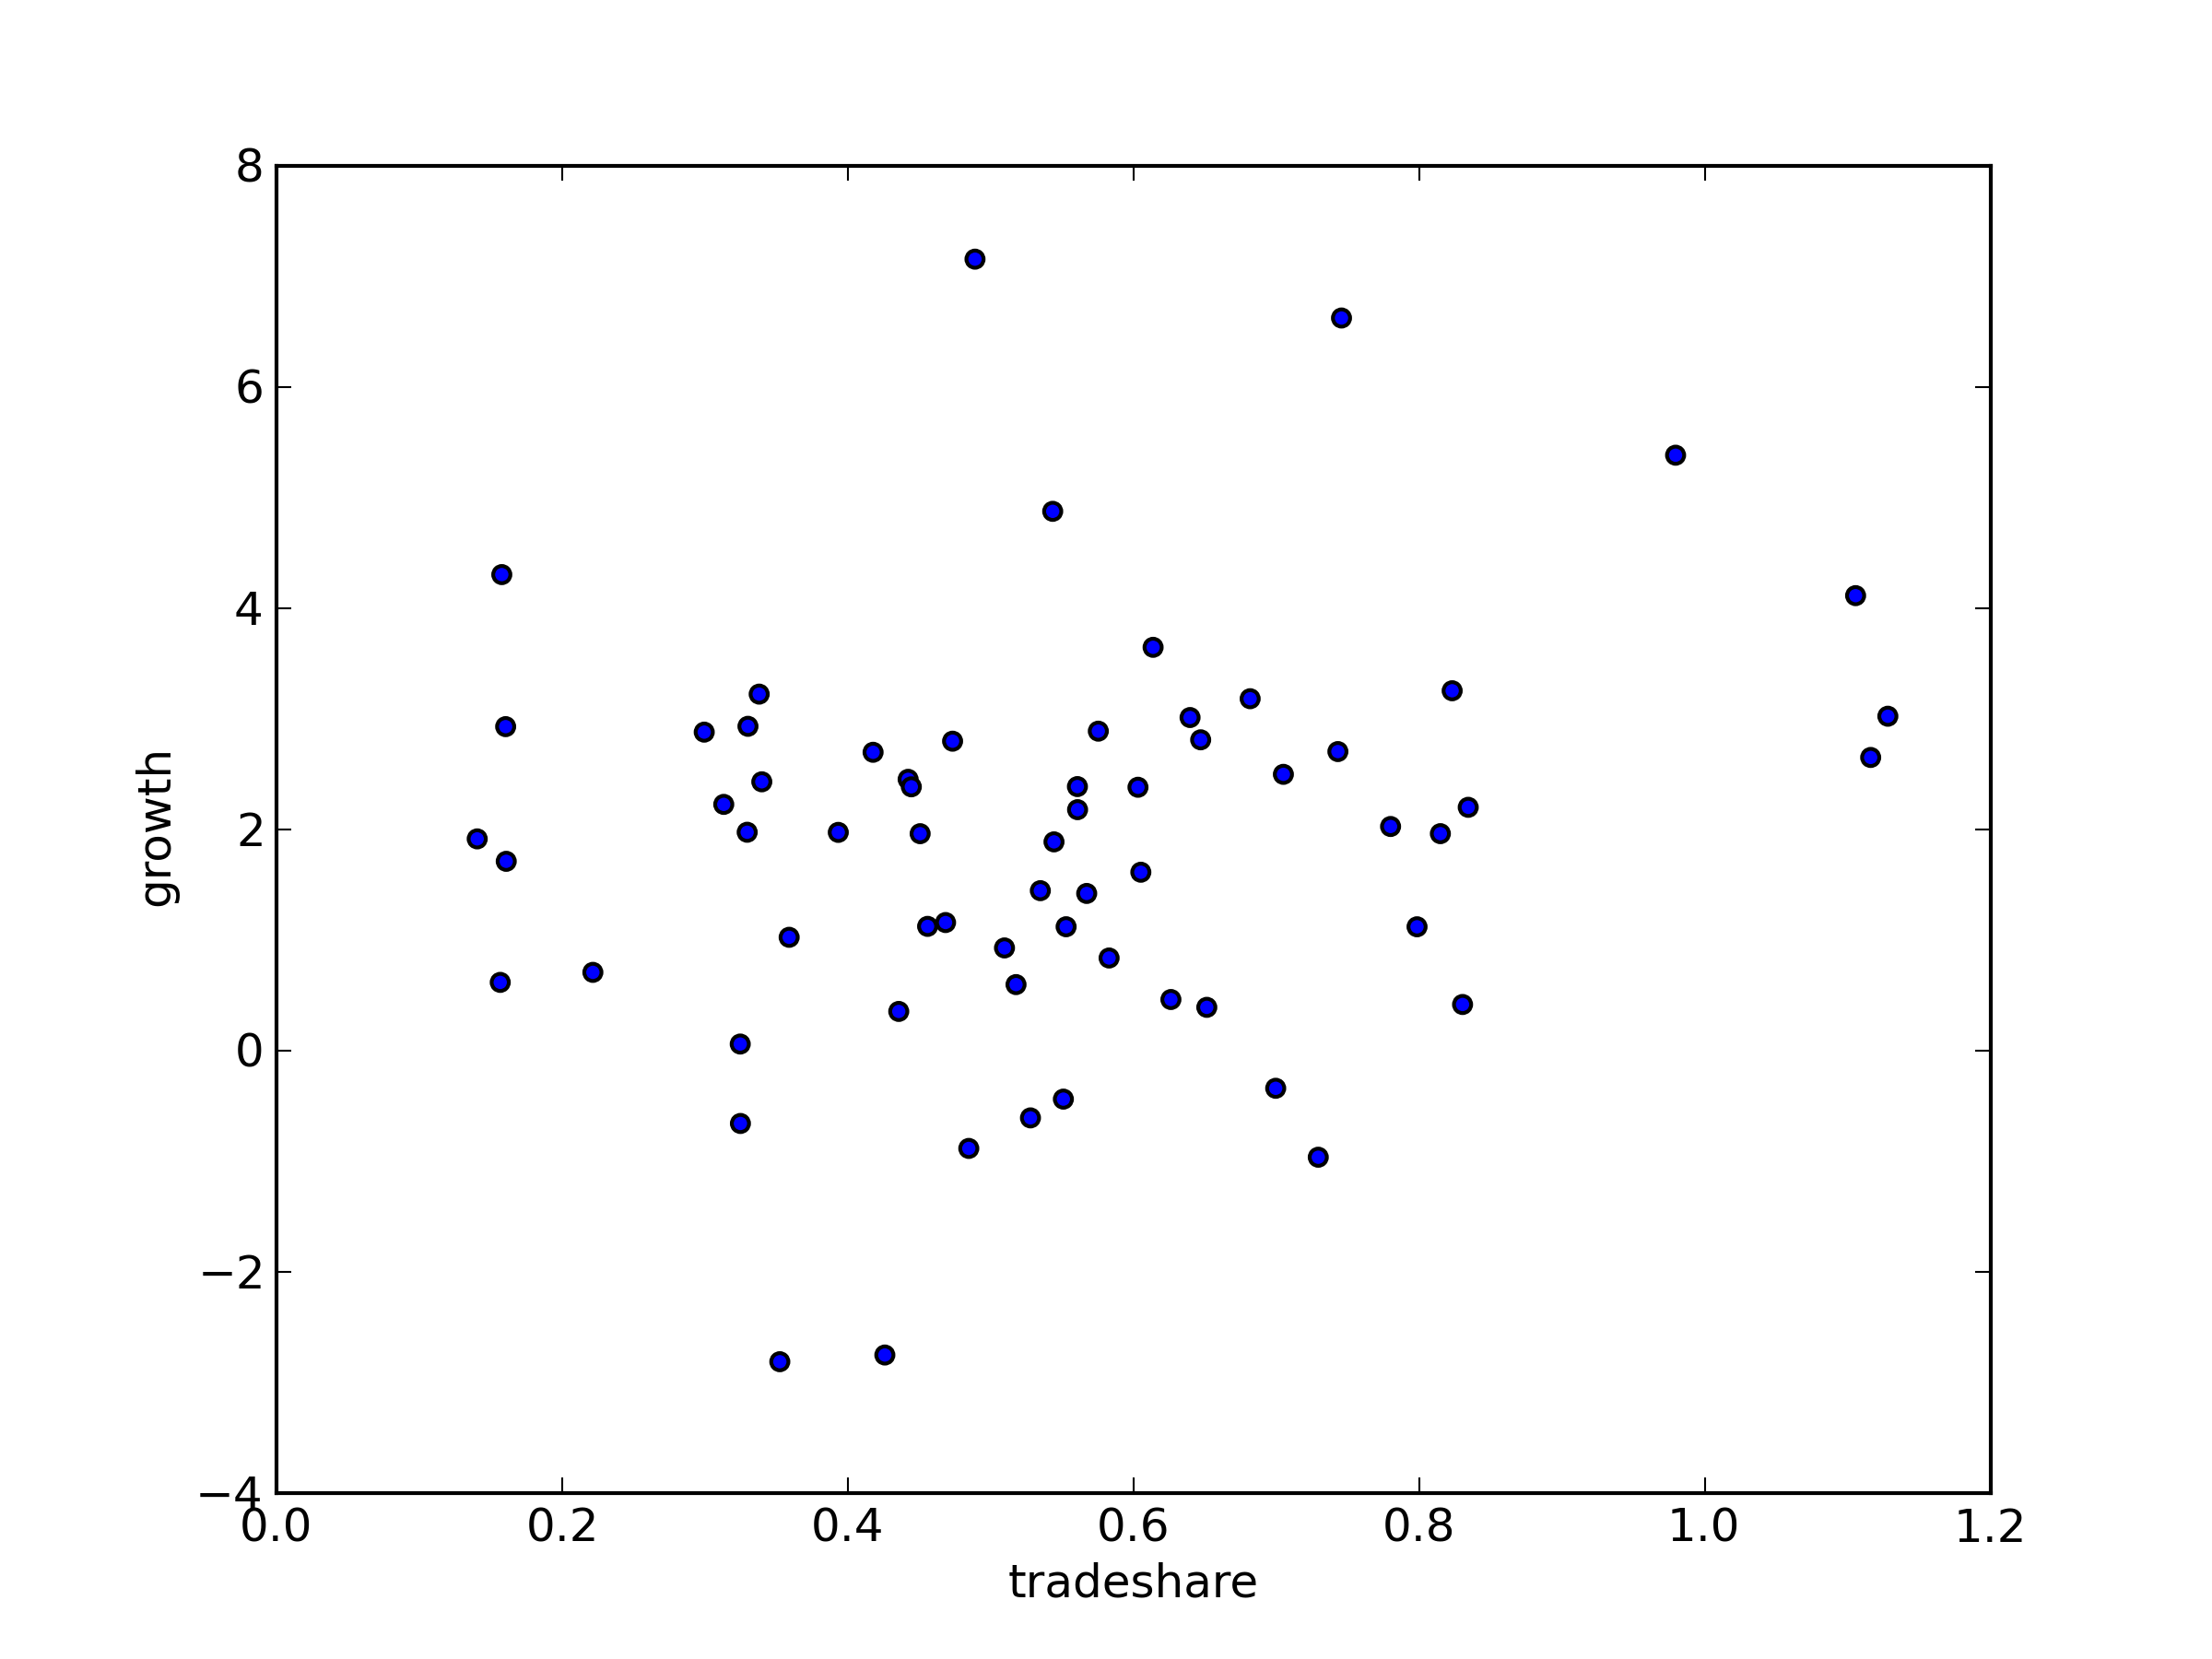
\includegraphics[scale = .33]{tradeGrowthScatter.png}

This relationship does not appear to be linear.  We seem to be missing other relevant variables, which is probably why the second regressions is better than the first.
\\

Part b.)

From regression 1, we'd expect Growth to increase by about $2 * 0.243 = .486$. 

From regression 2, we'd expect Growth to increase by about $ln(2) * 1.1063 = .7044$
\\

Part c.)

Individually, $Rev_Coups$ appears to be significant (t = -2.289) while $Assassinations$ does not (t = .0525).  Using robust errors, the t-statistics for $Rev_Coups$ and $Assassinations$ drop to .877092 and .319188.

Jointly, for the non-robust test the F statistic is 2.82796.  With 2 and 58 degrees of freedom, this gives a p-value of .06731.  The robust test gives an F of 3.4085 and a p-value of .03985.
\\

Part d.)

Regression 4 does not suggest that $TradeShare's$ effect is dependent upon $logSchool$ since the interaction variable is insignificant with a p-value of $0.168$.
\\

Part e.)

Regression 5 does not suggest a nonlinear relationship since the p-values for the square and cube of trade are both above 0.5.  There could of course still be nonlinear, just in a non-cubic form.
\\

Part f.)

From regression 3 we'd expect $Growth$ to increase by .55176.  From regression 5 we'd expect $Growth$ to \emph{decrease} by about 1.074.

\includegraphics[scale = .5]{mleResults.png}

\includegraphics[scale = .5]{part3OLS.png}
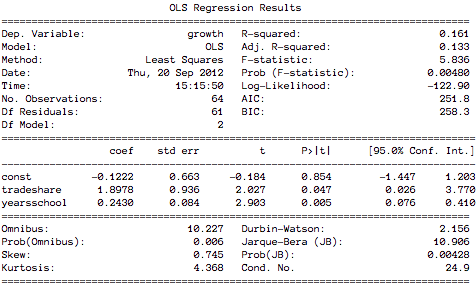
\includegraphics[scale = .5]{summary1.png}
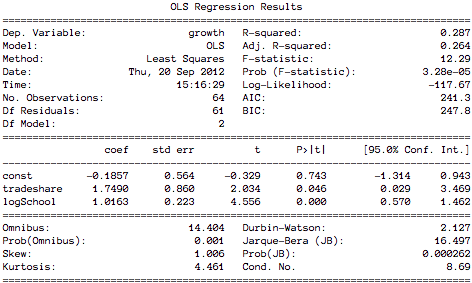
\includegraphics[scale = .5]{summary2.png}
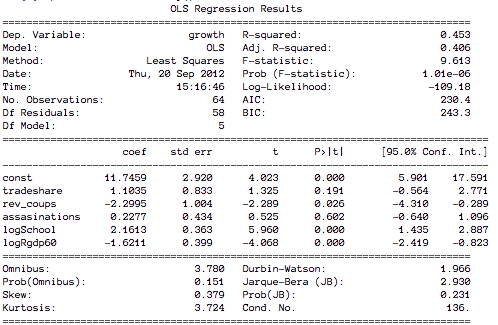
\includegraphics[scale = .5]{summary3.png}
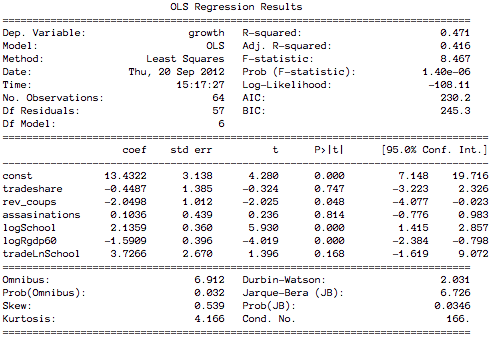
\includegraphics[scale = .5]{summary4.png}
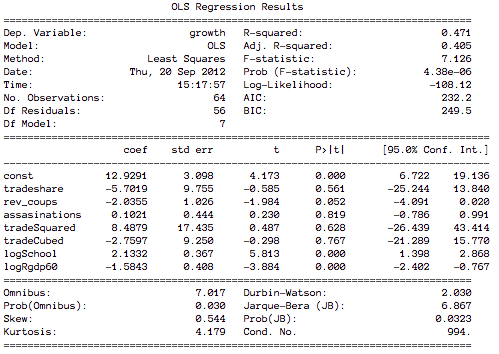
\includegraphics[scale = .5]{summary5.png}

I apologize for the terrible formatting.  Still working on a good way to get \LaTeX\ output.

The order going left to right, top to bottom:
\begin{itemize}
  \item Part 3b MLE
  \item Part 3b OLS
  \item Part 4, model 1, 2, 3, 4, 5
\end{itemize}

\end{document}